% Rodin Workshop 2016
% SCXML to iULM-B

\documentclass{llncs}

\newcommand{\specialcell}[2][c]{%
  \begin{tabular}[#1]{@{}c@{}}#2\end{tabular}}

 \newcommand{\myfigureshrinker}{\vspace{-1cm}}
 
\usepackage{doc}

\usepackage{abbrev}
\newabbrev[Rodin]{Rodin}{Rodin Platform}
\newabbrev{SCXML}{State Chart XML: State Machine Notation for Control Abstraction}
\newabbrev{EMF}{Eclipse Modelling Framework}

%use packages added by karla
\usepackage[utf8]{inputenc}
\usepackage[english]{babel}
\usepackage{color}
\usepackage{amsmath}
\usepackage{setspace}
\usepackage{fancyvrb,relsize}
\usepackage{aeguill}
\usepackage{rotating}
\usepackage{amssymb}
\usepackage{color}
\usepackage{amsbsy}
\usepackage{psfrag}
\usepackage{soul}
\usepackage{relsize}
\usepackage{verbatim}
%use packages added by karla

\newcommand{\miktex}{MiK{\TeX}}
\newcommand{\texniccenter}{{\TeX}nicCenter}
\newcommand{\makefile}{\texttt{Makefile}}
\newcommand{\latexeditor}{LEd}


\title{Translating SCXML Statecharts to iUML-B State-machines}

\author{
Karla Morris\inst{1}
\and
Colin Snook\inst{2}
}

\institute{
  Sandia National Laboratories, 
  Livermore, California, U.S.A.\\
  \email{knmorri@sandia.gov}
\and
   University of Southampton,
   Southampton, United Kingdom\\
   \email{cfs@ecs.soton.ac.uk}\\
 }

\authorrunning{}

\titlerunning{}

\begin{document}

\maketitle

\pagestyle{empty}

To facilitate automatic proof, the Event-B notation is restricted to a simple guarded action behaviour.
While iUML-B goes some way to provide an intuitive state-transition representation of Event-B models, its notation follows the semantics of Event-B.
Engineers that are used to the richer semantics of Harel style statecharts may find these restrictions difficult to accept.
Conversely, Event-B has features such as refinement and invariant properties that are not considered in most statechart notations.
It may be cumbersome for engineers to re-model existing systems into iUML-B for verification. 

  In order to explore the feasibility of this model transformation, we have developed a translation from a statechart representation, \SCXML \cite{scxmlwebsite}, into iUML-B. 
  For this initial work we do not support features of SCXML associated with more problematic areas of the semantic mismatch, such as `run to completion' transition sequencing. 
  Nevertheless, the translation provides an interesting first step towards interchange between the two notations.

 \SCXML is an XML notation for Harel (hence UML) style statecharts extended with a general purpose action language.
The concrete syntax for SCXML is based on XML  and includes a data modelling facility and an action language.
An example of SCXML syntax is shown in figure \ref{fig:scxml}.

To facilitate Event-B formal verification, extensions to the SCXML 
modelling notation are necessary so that additional modelling features 
required by Event-B can be integrated with the SCXML model.
The SCXML schema allows extension elements and attributes belonging 
to a different namespace to be added. 
The SCXML tooling provides fallback mechanisms so that these extensions are supported 
without the need for syntactic definition. We define a new namespace,  
\emph{iumlb} and add two new elements, \emph{iumlb:invariant} and 
\emph{iumlb:guard} as well as a 
number of new attributes.
Invariants are not supported in SCXML and SCXML transitions only have a single \emph{cond} attribute whereas we may need to introduce conjuncts of a transition
condition at various refinement steps. 
The concept  of refinement does not exist in SCXML. 
We introduce a new integer valued  attribute, \emph{iumlb:refinement}, which may be attached to any element of 
either namespace in order to specify the refinement level of that element. 

The iUML-B tools are based on the \EMF \cite{steinberg2009emf}. 
It is beneficial to load the SCXML model into EMF so that our existing model transformation technology can be used to implement the SCXML to iUML-B translation. 
An EMF meta-model for SCXML is available from the Sirius \cite{siriuswebsite} project. 
It supports generic model loading capabilities for new namespace extensions.
Hierarchical nested state charts are translated to similar corresponding  state-machine structures in iUML-B in a series of refinement levels as directed in the SCXML \emph{iumlb} extensions.  


\begin{figure}[tb!]
\myfigureshrinker
 \centering
\begin{minipage}[]{.8\textwidth}
        \fvset{frame=single,numbers=left,fontsize=\relsize{-10},numbersep=2pt}
          \VerbatimInput[samepage=false]{caseStudy/BlockState_Invariant.scxml}
          \caption{Part of SCXML model including iumlb extension elements} 
          \label{fig:scxml}
\end{minipage}
\end{figure}

\begin{figure}[tb!]
%\myfigureshrinker
 \centering
\begin{minipage}[]{.8\textwidth}
  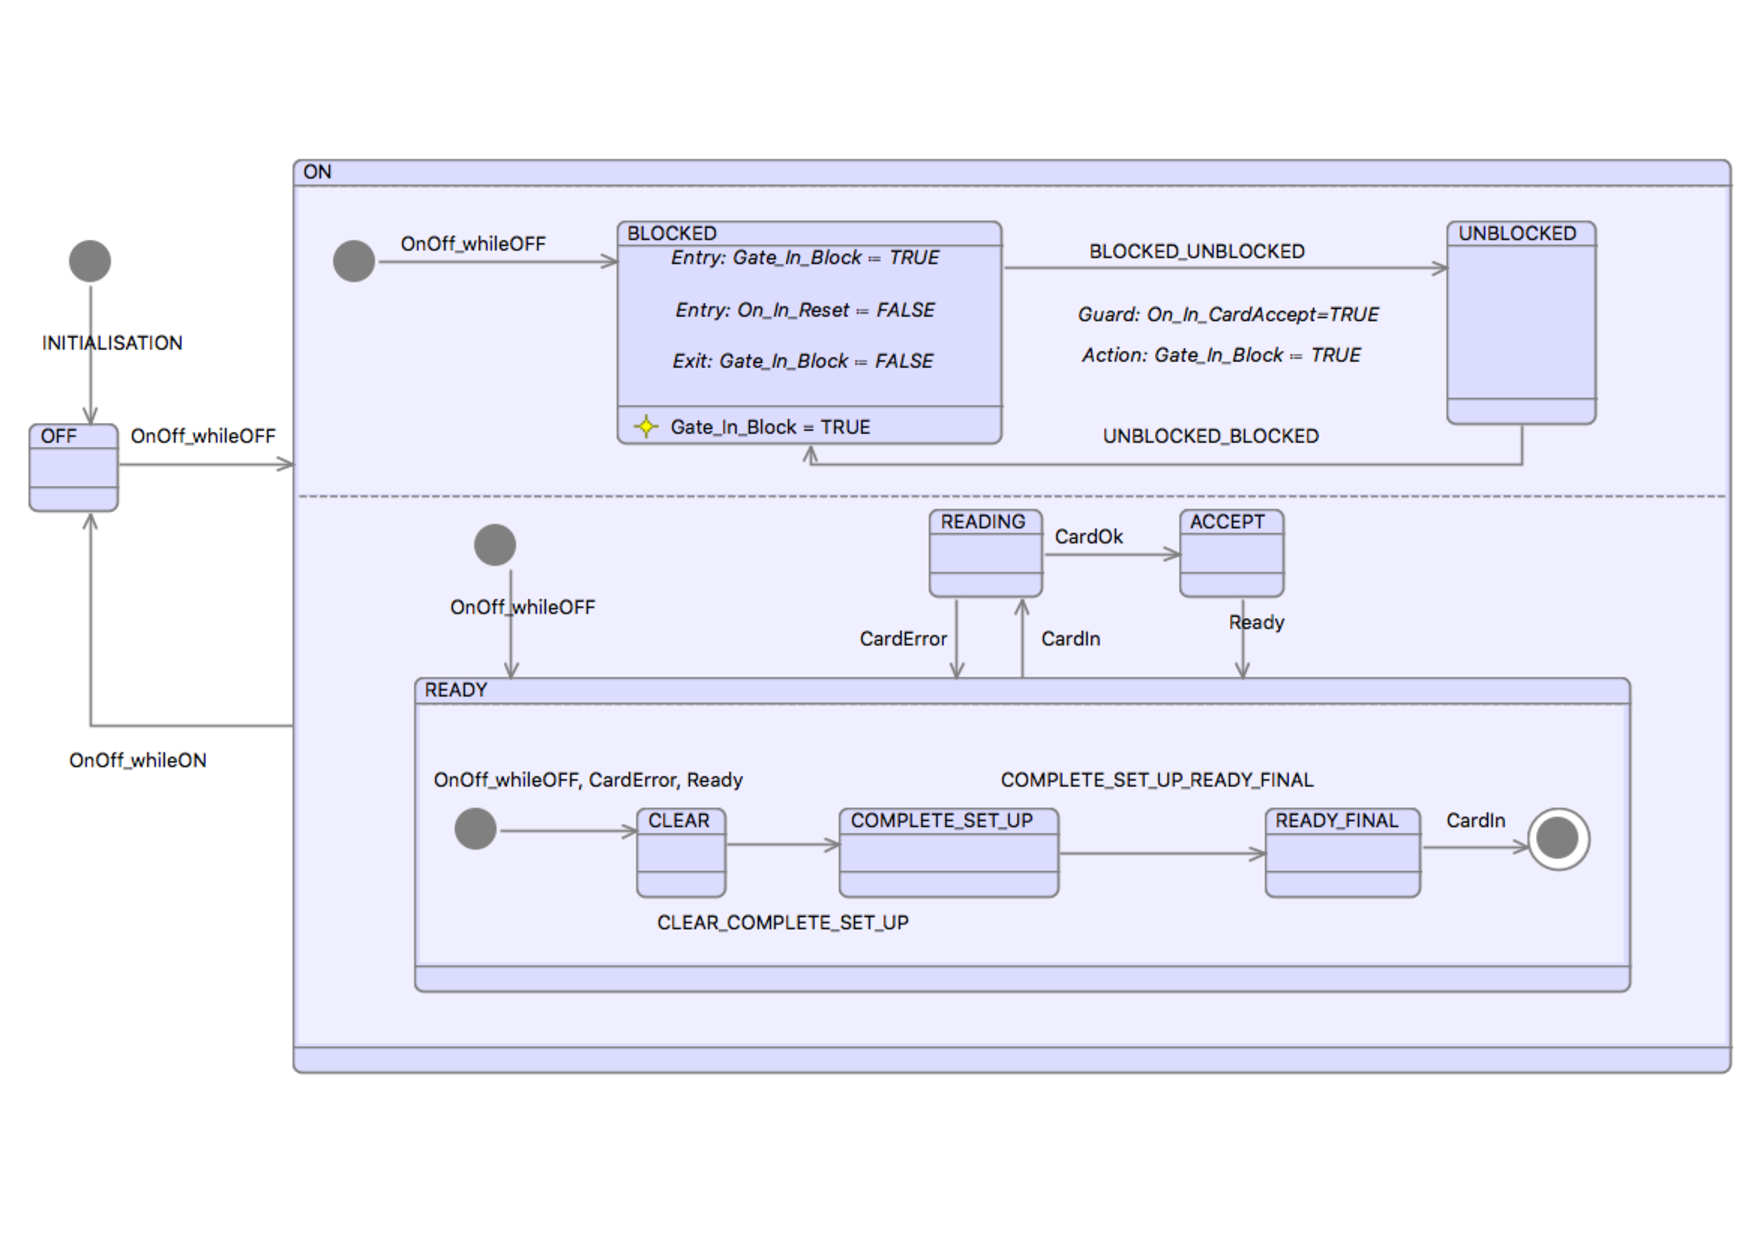
\includegraphics[width=1\textwidth]{caseStudy/TurnstileSimpleModel_iumlb}
  \caption{State-machine diagram in iUML-B at refinement level 3 (partially annotated with guards and actions)}
  \label{fig:StatemachineiUML-B}
\end{minipage}
\end{figure}


\bibliographystyle{plain}
\bibliography{main}

%------------------------------------------------------------------------------
\end{document}

